\documentclass[fleqn]{jsarticle}

\usepackage{graphicx}
\usepackage{amsmath,amssymb}
\usepackage{amsmath}
\usepackage{fancyhdr}

\pagestyle{fancy}
\fancyhead[RE,RO]{先端データ解析論 レポート}

\usepackage{xcolor}
\usepackage[justification=centering]{caption}
\usepackage{listings}
\renewcommand{\lstlistingname}{リスト}
\lstset{language=Python,%
        % basicstyle=\footnotesize,%
        basicstyle=\tiny,%
        commentstyle=\textit,%
        classoffset=1,%
        keywordstyle=\bfseries,%
      	frame=tRBl,framesep=5pt,%
      	showstringspaces=false,%
        linewidth=35em,
      	}%

\begin{document}

\title{先端データ解析論 第2回レポート}
\author{電子情報学専攻 48-176403 石毛真修}
\maketitle


\section*{大問1.}
$y = \frac{sin(\pi x)}{\pi x} + 0.1x + 0.2 \times random$ を ガウスカーネルモデル $f_\theta(x) = \sum_{j=1}^n \theta_j K(x_i, x_j)$
で近似し,更にそのハイパーパラメータである$\lambda$とカーネル関数の分散$h$を,交差確認法を使って決定する.

\begin{center}
\begin{tabular}{c}
  \begin{lstlisting}[caption=Regression Part,label=src_regression]
    import matplotlib.pyplot as plt
    import numpy as np


    def org_model(x):
      return np.sin(np.pi * x) / (np.pi * x) + 0.1 * x


    def get_samples(x_samples, f):
        return f(x_samples) + 0.2* np.random.randn(len(x_samples))


    def kern(x, c, h=0.2):
        norm = x - c
        return np.exp(- norm**2 / (2 * (h**2)))


    kerns = np.vectorize(kern)
    def kern_matrix(x_samples, h=0.2):
        return np.array([kerns(xi, x_samples, h) for xi in x_samples])


    def estimate_theta(samples_x, samples_y, lamb=1, h=0.2):
        K = kern_matrix(samples_x, h)
        Q = np.linalg.inv(np.matmul(K, K) + lamb * np.eye(len(samples_x)))
        p = np.matmul(np.transpose(K), samples_y)
        return np.matmul(Q, p)


    def kern_model_gen(x_samples, y_samples, lamb=1, h=0.2):
        est_theta = estimate_theta(x_samples, y_samples, lamb, h)
        def _model(x):
            return np.dot(est_theta, kerns(x, x_samples, h))
        v_model = np.vectorize(_model)
        return v_model


      np.random.seed()
      x_min, x_max = -3, 3
      n = 50
      N = 1000
      x = np.linspace(x_min, x_max, n)
      X = np.linspace(x_min, x_max, N)

      y = org_model(x)
      # _y = get_samples(x, org_model)

      lamb = 0.1
      h = 0.7
      est_model = kern_model_gen(x, _y, lamb, h)
      Y = est_model(X)

      plt.scatter(x, _y)
      plt.plot(x, y, 'r-', X, Y, 'b-')
      plt.show()
  \end{lstlisting}
\end{tabular}{c}
\end{center}

\begin{figure}[h]
  \begin{center}
    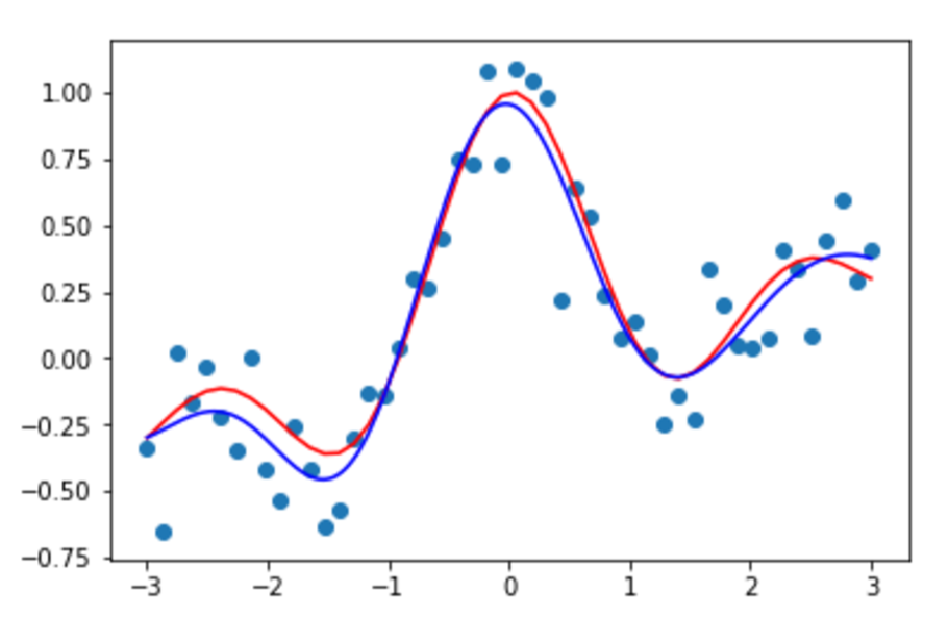
\includegraphics[width=0.6\textwidth]{figs/kernel_redge_basic.eps}
  \end{center}
  \caption{曲線 $y=\frac{sin(\pi x)}{\pi x} + 0.1x$ (赤)と $\lambda=0.1$, $h=0.7$ のときの回帰曲線(青).}
\end{figure}


\begin{center}
\begin{tabular}{c}
  \begin{lstlisting}[caption=Cross Validation and Grid Search,label=src_cross_validation]
    def split_train_test(x_samples, y_samples, k, i):
        batch_size = ceil(len(x_samples) / k)
        start_idx = i * batch_size
        end_idx = start_idx + batch_size
        if end_idx > len(x_samples):
            end_idx = len(x_samples)
        x_train = np.concatenate((
                x_samples[:start_idx], x_samples[end_idx:]))
        y_train = np.concatenate((
                y_samples[:start_idx], y_samples[end_idx:]))
        x_test = x_samples[start_idx:end_idx]
        y_test = y_samples[start_idx:end_idx]
        return x_train, x_test, y_train, y_test


    def cross_validation(x_samples, y_samples, model_gen, k=10):
        ave_err = 0
        for i in range(k):
            x_train, x_test, y_train, y_test =\
                    split_train_test(x_samples, y_samples, k, i)
            est_model = model_gen(x_train, y_train)
            diff = est_model(x_test) - y_test
            err = np.dot(diff, diff) / len(x_test)
            ave_err += err
        ave_err /= k
        return ave_err


    def grid_search(model_gen, x_samples, y_samples, l_search_points,
                    h_search_points):
        err_min = 10000
        likely_solution = [np.nan, np.nan]
        grid_err = np.zeros((len(h_search_points), len(l_search_points)))
        for i, l in enumerate(l_search_points):
            for j, h in enumerate(h_search_points):
                def _model_gen(x, y):
                    return model_gen(x, y, l, h)
                err = cross_validation(x_samples, y_samples, _model_gen)
                grid_err[j, i] = err
                if err < err_min:
                    err_min = err
                    likely_solution = [l, h]
        return err_min, likely_solution, grid_err


    l_search_points = np.logspace(-2, 3, 6)
    h_search_points = np.linspace(0.001, 2, 50)

    err_min, params, grid_err = grid_search(
      kern_model_gen, x, _y, l_search_points, h_search_points)

    from mpl_toolkits.mplot3d import Axes3D
    import matplotlib.pyplot as plt

    X, Y = np.meshgrid(l_search_points, h_search_points)
    fig = plt.figure()
    ax = Axes3D(fig)
    ax.set_xlabel('Lambda')
    ax.set_ylabel('h')
    ax.set_zlabel('Square Error')

    ax.plot_surface(X, Y, grid_err, rstride=1, cstride=1)
    plt.show()
  \end{lstlisting}
\end{tabular}{c}
\end{center}

\noindent
このコードを実行することにより,$\lambda=0.1$,$h=0.78$のとき平均誤差が 0.0374637682683 となるような回帰曲線が得られた.

\begin{figure}[h]
  \begin{center}
    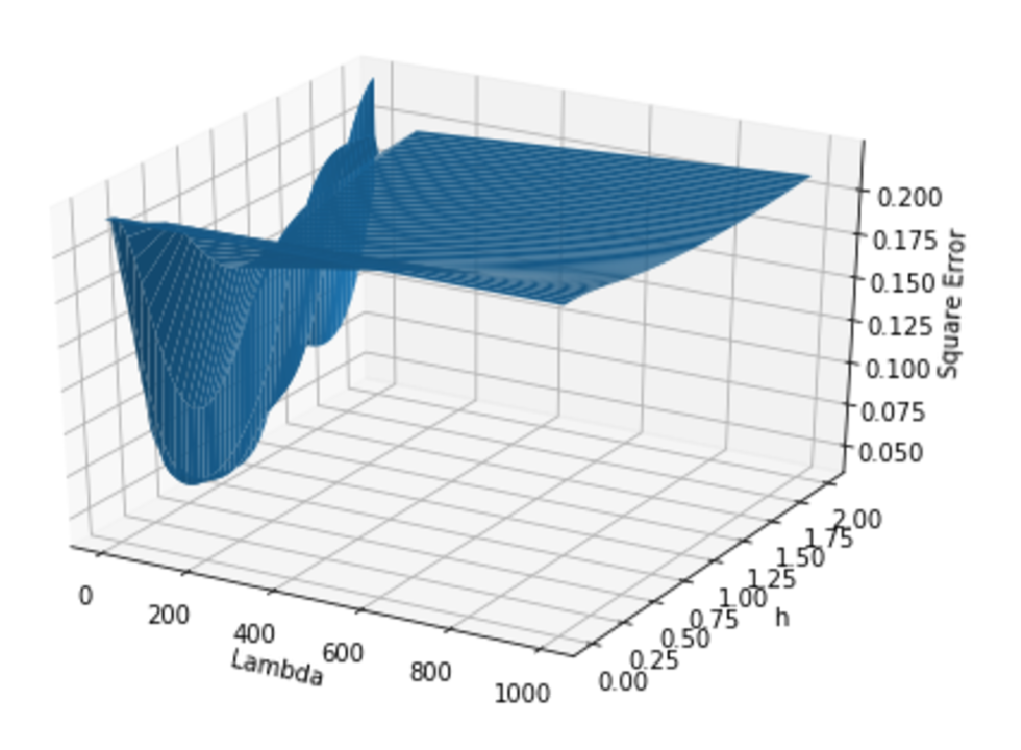
\includegraphics[width=0.8\textwidth]{figs/cross_validation.eps}
  \end{center}
  \caption{グリッドサーチの結果}
\end{figure}



\section*{大問2.}
線形モデル $f_\theta = \sum_{j=1}^b \theta_j \phi_j(\mathbf{x})$ を用いた$l_2$-正則化回帰に対する
ひとつ抜き交差確認による二乗誤差が,次のようになることを示す.
\begin{equation*}
  \frac{1}{n} \| \tilde{\mathbf{H}}^{-1} \mathbf{H} \mathbf{y} \|^2
\end{equation*}

\subsection*{導出}
  標本 $(\mathbf{x}_i, y_i)$ を除いて学習したパラメータ $\hat{\mathbf{\theta}_i}$ は次のように表される.

  \begin{equation*}
    \hat{\mathbf{\theta}_i} = (\mathbf{\Phi}_i^\mathrm{T} \mathbf{\Phi}_i + \lambda \mathbf{I})^{-1} \mathbf{\Phi}_i^\mathrm{T} \mathbf{y}_i
    = \mathbf{U}_i^{-1} \mathbf{\Phi}_i^\mathrm{T} \mathbf{y}_i
  \end{equation*}

  \begin{eqnarray*}
    \mathbf{U}_i &=& \mathbf{\Phi}_i^\mathrm{T} \mathbf{\Phi}_i + \lambda \mathbf{I}\\
    &=& \mathbf{\Phi}^\mathrm{T} \mathbf{\Phi} - \mathbf{\phi}_i \mathbf{\phi}_i^\mathrm{T} + \lambda \mathbf{I}\\
    &=& (\mathbf{\Phi}^\mathrm{T} \mathbf{\Phi} + \lambda \mathbf{I})- \mathbf{\phi}_i \mathbf{\phi}_i^\mathrm{T} \\
  \end{eqnarray*}

  であるので,
  \begin{eqnarray*}
    \mathbf{U}_i^{-1} &=& \{ (\mathbf{\Phi}^\mathrm{T} \mathbf{\Phi} + \lambda \mathbf{I}) - \mathbf{\phi}_i \mathbf{\phi}_i^\mathrm{T} \}^{-1}\\
    &=& (\mathbf{\Phi}^\mathrm{T} \mathbf{\Phi} + \lambda \mathbf{I})^{-1} +
      \frac{(\mathbf{\Phi}^\mathrm{T} \mathbf{\Phi} + \lambda \mathbf{I})^{-1} \mathbf{\phi}_i \mathbf{\phi}_i^\mathrm{T} (\mathbf{\Phi}^\mathrm{T} \mathbf{\Phi} + \lambda \mathbf{I})^{-1}}
        {1 - \mathbf{\phi}_i^\mathrm{T} (\mathbf{\Phi}^\mathrm{T} \mathbf{\Phi} + \lambda \mathbf{I})^{-1} \mathbf{\phi}_i}\\
    &=& \mathbf{U}^{-1} + \frac{\mathbf{U}^{-1} \mathbf{\phi}_i \mathbf{\phi}_i^\mathrm{T} \mathbf{U}^{-1}}{\gamma_i}
  \end{eqnarray*}

  ただし,
  \begin{equation*}
    \gamma_i = 1 - \mathbf{\phi}_i^\mathrm{T} (\mathbf{\Phi}^\mathrm{T} \mathbf{\Phi} + \lambda \mathbf{I})^{-1} \mathbf{\phi}_i
  \end{equation*}

  以上から,
  \begin{eqnarray*}
    \hat{\mathbf{\theta}_i} = \left\{ \mathbf{U}^{-1} + \frac{\mathbf{U}^{-1} \mathbf{\phi}_i \mathbf{\phi}_i^\mathrm{T} \mathbf{U}^{-1}}{\gamma_i} \right\}
      (\mathbf{\Phi}^\mathrm{T} \mathbf{y} - \mathbf{\phi}_i y_i)
    = \left\{ \mathbf{U}^{-1} + \frac{\mathbf{U}^{-1} \mathbf{\phi}_i \mathbf{\phi}_i^\mathrm{T} \mathbf{U}^{-1}}{\gamma_i} \right\}
      \left( \sum_{j \neq i}^b y_j \mathbf{\phi}_j \right)
  \end{eqnarray*}

  一方で最終的な誤差 $E$ は,
  \begin{eqnarray*}
    E = \frac{1}{n} \sum_i^n \left(\mathbf{\phi}_i^\mathrm{T} \hat{\mathbf{\theta}_i} - y_i \right)^2
  \end{eqnarray*}

  \begin{eqnarray*}
    \mathbf{\phi}_i^\mathrm{T} \hat{\mathbf{\theta}_i} - y_i &=&
      \mathbf{\phi}_i^\mathrm{T} \left\{ \mathbf{U}^{-1} + \frac{\mathbf{U}^{-1} \mathbf{\phi}_i \mathbf{\phi}_i^\mathrm{T} \mathbf{U}^{-1}}{\gamma_i} \right\}
      \left( \sum_{j \neq i}^b y_j \mathbf{\phi}_j \right) - y_i\\
    &=& \left\{ \mathbf{\phi}_i^\mathrm{T} \mathbf{U}^{-1} + \frac{\mathbf{\phi}_i^\mathrm{T} \mathbf{U}^{-1} \mathbf{\phi}_i \mathbf{\phi}_i^\mathrm{T} \mathbf{U}^{-1}}{\gamma_i} \right\}
      \left( \sum_{j \neq i}^b y_j \mathbf{\phi}_j \right) - y_i\\
    &=& \left( 1 + \frac{1-\gamma_i}{\gamma_i} \right) \mathbf{\phi}_i^\mathrm{T} \mathbf{U}^{-1} \left( \sum_{j \neq i}^b y_j \mathbf{\phi}_j \right) - y_i\\
    &=& \frac{1}{\gamma_i} \mathbf{\phi}_i^\mathrm{T} \mathbf{U}^{-1} \left( \sum_{j \neq i}^b y_j \mathbf{\phi}_j \right) - y_i\\
    &=& - \left( y_i - \sum_{j \neq i}^b y_j \frac{ \mathbf{\phi}_i^\mathrm{T} \mathbf{U}^{-1} \mathbf{\phi}_j }{\gamma_i} \right)
  \end{eqnarray*}

  よって,
  \begin{eqnarray*}
    nE = \sum_i^n \left( y_i - \sum_{j \neq i}^b y_j \frac{ \mathbf{\phi}_i^\mathrm{T} \mathbf{U}^{-1} \mathbf{\phi}_j }{\gamma_i} \right)^2
  \end{eqnarray*}

  \vspace{10em}
  \begin{eqnarray*}
    \mathbf{H} = \mathbf{I} - \mathbf{\Phi} \mathbf{U}^{-1} \mathbf{\Phi}^\mathrm{T}\ \ \ \ \
    \tilde{H}_{ii} = 1 - \mathbf{\phi}_i^\mathrm{T} \mathbf{U}^{-1} \mathbf{\phi}_i = \gamma_i
  \end{eqnarray*}

  であるので,
  \begin{eqnarray*}
    \tilde{\mathbf{H}}^{-1} \mathbf{H} \mathbf{y} &=&
      \begin{bmatrix}
        1 &-\frac{\mathbf{\phi}_1^\mathrm{T} \mathbf{U}^{-1} \mathbf{\phi}_2}{\gamma_1}
          &-\frac{\mathbf{\phi}_1^\mathrm{T} \mathbf{U}^{-1} \mathbf{\phi}_3}{\gamma_1}
          & ...
          &-\frac{\mathbf{\phi}_1^\mathrm{T} \mathbf{U}^{-1} \mathbf{\phi}_n}{\gamma_1}\\
        -\frac{\mathbf{\phi}_2^\mathrm{T} \mathbf{U}^{-1} \mathbf{\phi}_1}{\gamma_2}
          & 1
          &-\frac{\mathbf{\phi}_2^\mathrm{T} \mathbf{U}^{-1} \mathbf{\phi}_3}{\gamma_2}
          & ...
          &-\frac{\mathbf{\phi}_2^\mathrm{T} \mathbf{U}^{-1} \mathbf{\phi}_n}{\gamma_2}\\
        &.\\&&.\\&&&.\\
        -\frac{\mathbf{\phi}_n^\mathrm{T} \mathbf{U}^{-1} \mathbf{\phi}_1}{\gamma_2}
        & ...
        & ...
        & ...
        & 1\\
      \end{bmatrix}
      \mathbf{y}\\ \\ \\
    &=&
      \begin{bmatrix}
        y_1 - \sum_{j \neq 1}^b y_j \frac{ \mathbf{\phi}_1^\mathrm{T} \mathbf{U}^{-1} \mathbf{\phi}_j }{\gamma_1}\\
        y_2 - \sum_{j \neq 2}^b y_j \frac{ \mathbf{\phi}_2^\mathrm{T} \mathbf{U}^{-1} \mathbf{\phi}_j }{\gamma_2}\\
        .\\
        .\\
        .\\
        y_n - \sum_{j \neq n}^b y_j \frac{ \mathbf{\phi}_n^\mathrm{T} \mathbf{U}^{-1} \mathbf{\phi}_j }{\gamma_n}\\
      \end{bmatrix}
  \end{eqnarray*}

  以上から,
  \begin{eqnarray*}
    \| \tilde{\mathbf{H}}^{-1} \mathbf{H} \mathbf{y} \|^2 = \sum_i^n \left( y_i - \sum_{j \neq i}^b y_j \frac{ \mathbf{\phi}_i^\mathrm{T} \mathbf{U}^{-1} \mathbf{\phi}_j }{\gamma_i} \right)^2 = nE
  \end{eqnarray*}

\end{document}
